%package list
\documentclass{article}
\usepackage[top=3cm, bottom=3cm, outer=3cm, inner=3cm]{geometry}
\usepackage{graphicx}
\usepackage{url}
%\usepackage{cite}
\usepackage{hyperref}
\usepackage{array}
\usepackage{multicol}
\newcolumntype{x}[1]{>{\centering\arraybackslash\hspace{0pt}}p{#1}}
\usepackage{natbib}
\usepackage{pdfpages}
\usepackage{float}
\usepackage{multirow}
\usepackage[normalem]{ulem}
\useunder{\uline}{\ul}{}

\usepackage[english,spanish]{babel}
\usepackage[utf8]{inputenc}
\AtBeginDocument{\selectlanguage{spanish}}
\renewcommand{\figurename}{Figura}
\renewcommand{\refname}{Referencias}
\renewcommand{\tablename}{Tabla} %esto no funciona cuando se usa babel
\AtBeginDocument{%
	\renewcommand\tablename{Tabla}
}

\usepackage{fancyhdr}
\pagestyle{fancy}
\fancyhf{}
\setlength{\headheight}{30pt}
\renewcommand{\headrulewidth}{1pt}
\renewcommand{\footrulewidth}{1pt}
\fancyhead[L]{\raisebox{-0.2\height}{
\includegraphics[width=3cm]{img/logo_innovate}}}
\fancyhead[C]{}
\fancyhead[R]{\fontsize{12}{12}\selectfont	Convenio N$^{\circ}$ 165-INNOVATEPERU-PIEC1-2019}
\fancyfoot[L]{SISO}
\fancyfoot[C]{IIDSVA}
\fancyfoot[R]{Página \thepage}




\begin{document}
	
	\begin{center}	
		\fontsize{15}{15} \textbf{Informe de pruebas SISO-VID}
	\end{center}
	%\centerline{\textbf{\underline{\Large Título: Informe de revisión del estado del arte}}}
	%\vspace*{0.5cm}
	
	\begin{table}[h]
		\setlength{\tabcolsep}{0.5em} % for the horizontal padding
		{\renewcommand{\arraystretch}{1.6}% for the vertical padding
			\begin{tabular}{|p{4cm}|p{10.8cm}|}
				\hline 
				\textbf{Elaboración:} & Equipo técnico  \\	\hline 
				\textbf{Entidad Ejecutora:} & X-TRA PLUS SOLUCIONES DE ENERGÍA S.A.C  \\	\hline 
				\textbf{Proyecto:} & Desarrollo de un Sistema Adaptativo para la Detección de Somnolencia en Conductores de Transporte Interprovincial idóneo para las características únicas de las Carreteras del Perú mediante Sensado Híbrido utilizando Técnicas de Deep Learning.  \\	\hline 
				\textbf{Periodo:} & Marzo 2021  \\	\hline 
				\textbf{Fecha:} & \today  \\	\hline 
			\end{tabular}
		}
	\end{table}	
	
	
	
	\section{Objetivo}
	
	Realizar las pruebas del modulo SISO-VID. Este componente de software es el encargado de detectar somnolencia a partir de una secuencia de video utilizando aprendizaje profundo.
	
	\section{Introducción}
	
	Según \textit{World Health Organization} \cite{who}, 1.24 millones de accidentes de tráfico ocurren cada día. Además, \textit{The National Highway Traffic Safety Administration} (NHTSA), menciono que en USA han ocurrido 153,297 accidentes de transito entre el 2011 al 2015, y de estos el 2.4\%  fueron causados por conductres con somnolencia. Incluso, 1.25 millones de personas mueren cada año en accidentes de transito, 20 a 50 millones han sido heridos o estan discapacitados y todo esto ha llegado a costar 518 billones de dolares. Mas alarmante, se predice que los accidentes de transito serán la quinta causa mas frecuente de muertes para el 2030 \citep{asirt}. \\	
	
	SISO-VID toma como entrada una secuencia de video y dectada si alguna escena de la secuencia de video presenta somnolencia. En resumen, se ha utilizado detección de rostros con una red neuronal \textit{Single Shot Detector} (SSD), luego sobre el rostro detectado se evaluaron tres modelos de redes neuronales (VGG, ResNet e Inception) para determinar la de mejor desempeño, de estas se escogio la red neuronal Inception. 
	
	
	
	\section{SISO-VID} \label{desarrollo}
	
	SISO-VID es un componente de software basado en aprendizaje profundo para la detección de somnolencia tomando como entrada una secuencia de video. En la Figura \ref{fig:siso_vid}, presentamos la metodología utilizada de SISO-VID. El método propuesto toma una secuencia de video como entrada, luego extrae los fotogramas, por cada fotograma se detecta el rostro utilizando la red neuronal SSD, para finalmente utilizar la red Inception sobre el rostro detectado para determinar si exista somnolencia. En la ultima etapa, se utilizó Inception al ser la de mejor acierto comparado con VGG y ResNet.\\
	
	\begin{figure}[H]
		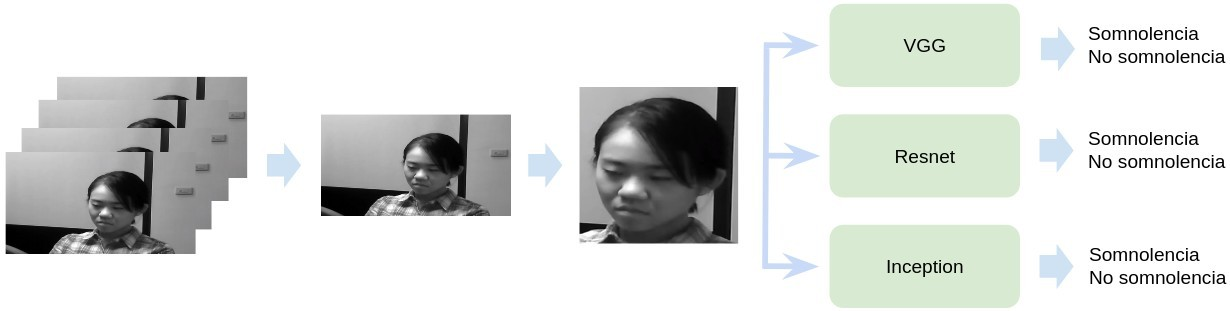
\includegraphics[width=\textwidth]{img/siso_vid}		
		\caption{Metodología utilizada por SISO-VID.}
		\label{fig:siso_vid}
	\end{figure}

	
	\subsection{VGG}
	
	Propuesta por \cite{simonyan2014very} en el 2014, es una de las primeras redes profundas más conocida. VGG tiene varias versiones diferenciadas por el número de capas, entre esta tenemos VGG-16 y VGG-19. En la Figura \ref{fig:vgg16} y \ref{fig:vgg19}, detallamos la arquitectura de VGG-16 y VGG-19 respectivamente. Nosotros evaluamos el desempeño de VGG-19 para la detección de somnolencia.
	
	\begin{figure}[H]
		\centering
		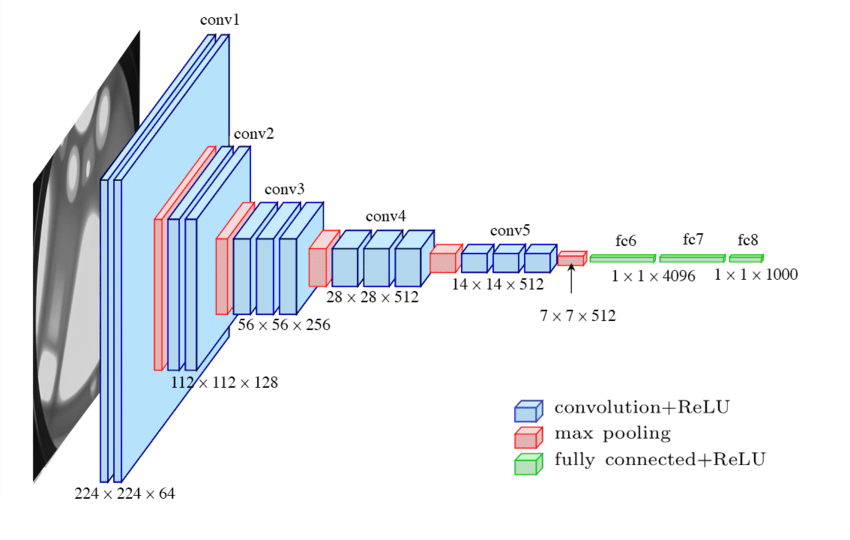
\includegraphics[width=0.7\textwidth]{img/vgg16}		
		\caption{Arquitectura de la red neuronal VGG-16.}
		\label{fig:vgg16}
	\end{figure} 
	\begin{figure}[H]
		\centering
		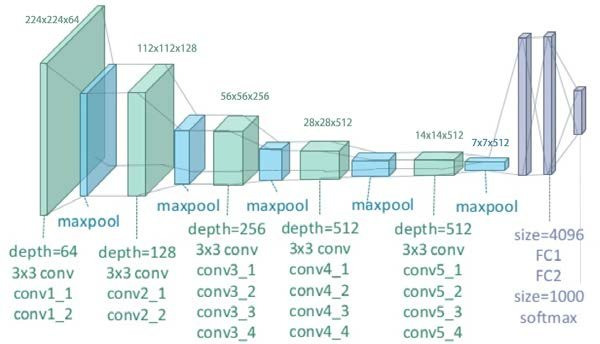
\includegraphics[width=0.68\textwidth]{img/vgg19}		
		\caption{Arquitectura de la red neuronal VGG-19.}
		\label{fig:vgg19}
	\end{figure}

	Los parametros e hyper parametros utilizados para esta red neuronal VGG-19 se presentan en la Tabla \ref{tab:vgg}.
	
	\begin{table}[h]
		\centering		
		\caption{Parametros utilizados con VGG-19}
		\label{tab:vgg}
		\begin{tabular}{ p{3cm} p{3cm}}
			\hline 
			\textbf{Parametro} & \textbf{Valor}   \\
			\hline 
			batch & 32 \\
			input & 224 x 224 x 3 \\
			momentum & 0.9 \\
			decay & 0.0005 \\
			learning rate & 0.001 \\
			epochs & 100 \\
			\hline 
		\end{tabular}
	\end{table}
	
	\subsection{ResNet}

	Propuesta por \cite{he2016deep}, representa un gran avance en computación gráfica en los ultimos años. ResNet, hizo posible entrenar cientos de capas de neuronas y lograr buenos resultados. La idea principal de ResNet es la introducción del concepto \textit{identity shortcut connection}, que salta una o mas capas (ver Figura \ref{fig:resnet1}). Con este concepto, los autores solucionaron el problema de \textit{vanish gradient} que se tenia en arquitecturas grandes de redes. En la Figura \ref{fig:resnet2}, mostramos una compración de ResNet con VGG-19 y otra red con 34 capas (SISO-VID utilizo dicha arquitectura de ResNet).

	\begin{figure}[H]
		\centering
		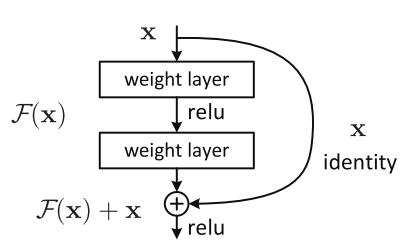
\includegraphics[width=0.4\textwidth]{img/resnet1}		
		\caption{Bloque residual utilizado por ResNet.}
		\label{fig:resnet1}
	\end{figure} 

\begin{figure}[H]
	\centering
	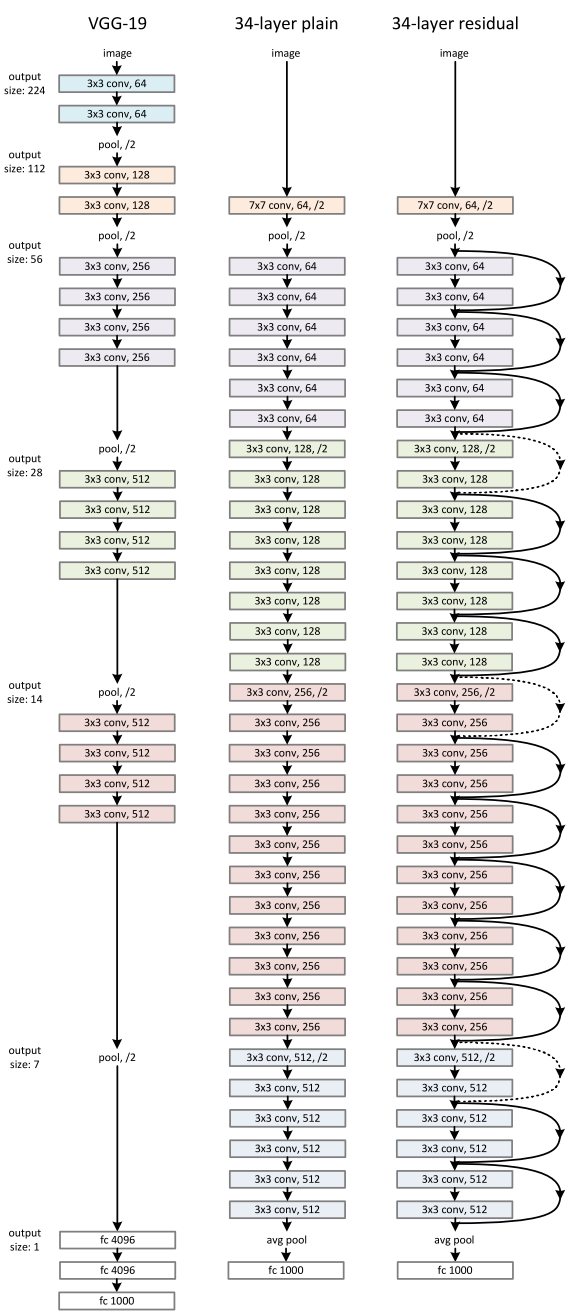
\includegraphics[width=0.6\textwidth]{img/resnet2}		
	\caption{Arquitectura de ResNet utilizada y una comparación con VGG-19 y una red con 34 capas.}
	\label{fig:resnet2}
\end{figure} 

	Los parametros e hyper parametros utilizados para esta red neuronal ResNet se presentan en la Tabla \ref{tab:resnet}.
	
	\begin{table}[h]
		\centering		
		\caption{Parametros utilizados con ResNet}
		\label{tab:resnet}
		\begin{tabular}{ p{3cm} p{3cm}}
			\hline 
			\textbf{Parametro} & \textbf{Valor}   \\
			\hline 
			batch & 32 \\
			input & 224 x 224 x 3 \\
			momentum & 0.9 \\
			decay & 0.0005 \\
			learning rate & 0.001 \\
			epochs & 100 \\
			\hline 
		\end{tabular}
	\end{table}


	\subsection{Inception}
	
	La red neuronal Inception \cite{szegedy2016rethinking} en su tercera versión, es un modelo de reconocimiento de imágenes muy utilizado, está logró una exactitud de 78.1\% en la base de datos ImageNet. Debido a esto, se utilizo esta red neuronal para detectar somnolencia. \\
	
	La red neuronal Inception-v3 hace uso de unos módulos llamados Inception. Estos actúan como filtros aplicados a un mismo valor de entrada mediante capas convolucionales y de \textit{pooling}. Esto permite sacar provecho de la extracción de patrones que brindan diferentes tamaños en los filtros. Luego, el resultado de estos filtros es concatenado y utilizado como el valor de salida del módulo. Este modelo aumenta el número de parámetros entrenables y la computación requerida, pero mejora considerablemente la exactitud. En la Figura \ref{fig:inception}, mostramos la arquitectura de esta red.
	
	
	
	\begin{figure}[H]
		\centering
		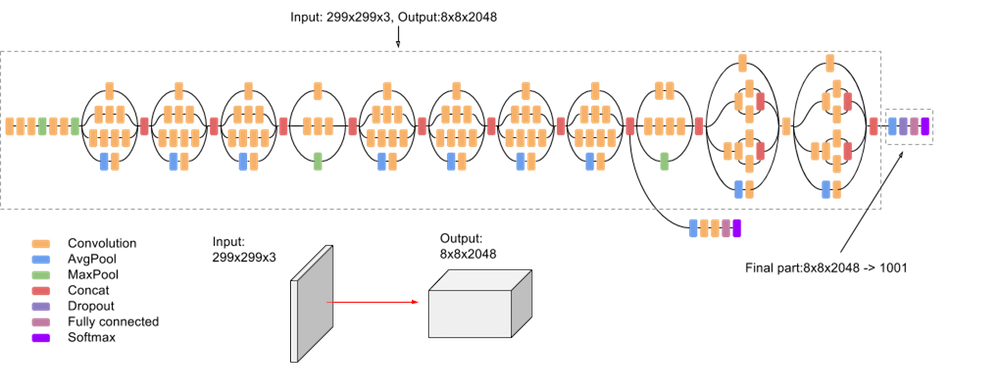
\includegraphics[width=\textwidth]{img/inception}		
		\caption{Detección de somnolencia a partir de un rostro utilizando VGG, Resnet e Inception.}
		\label{fig:inception}
	\end{figure}

	Los parametros e hyper parametros utilizados para esta red neuronal se presentan en la Tabla \ref{tab:inception}.
	
	\begin{table}[H]
		\centering		
		\caption{Parametros utilizados con Inception-v3}
		\label{tab:inception}
		\begin{tabular}{ p{3cm} p{3cm}}
			\hline 
			\textbf{Parametro} & \textbf{Valor}   \\
			\hline 
			batch & 32 \\
			input & 224 x 224 x 3 \\
			momentum & 0.9 \\
			decay & 0.0005 \\
			learning rate & 0.001 \\
			epochs & 100 \\
			\hline 
		\end{tabular}
	\end{table}

	\section{Pruebas}
	
	Para el entrenamiento de las tres redes neuronales se utilizó tres bases de datos:
	
	\begin{itemize}
		\item \textbf{NTHU}.- Propuesta por \cite{weng2016driver}, esta base de datos contiene videos de personas con somnolencia. Lamentablemente, los videos no son de conductores reales, al contrario, son actores en una oficina con buenas condiciones de iluminación.
		\item \textbf{SISO-IMG}.- En el proyecto se construyo esta base de datos de varios videos recolectados de una empresa de transporte. A diferencia de NTHU, esta base de datos contiene videos de conductores reales durante su jornada laboral.
		\item \textbf{SISO-NTHU}.- Esta es la unión de la base de datos NTHU y SISO-IMG.		
	\end{itemize}

	En la Tabla \ref{tab:bds}, detallamos la cantidad de muestras por clase de cada base de datos. En este caso, la base de datos SISO-IMG, tiene pocas muestras debido a las pocas grabaciones que se hizo en la empresa de transporte (debido a la pandemia causada por el COVID-19).
	
	\begin{table}[H]
		\centering		
		\caption{Cantidad de muestras por clase y base de datos utilizadas en los experimentos.}
		\label{tab:bds}
		\begin{tabular}{ p{3cm} p{3cm} p{3cm}}
			\hline 
			\textbf{Base de datos} & \textbf{Dormido} & \textbf{Despierto}   \\
			\hline 
			NTHU & 8995 & 8995 \\
			SISO-IMG & 933 & 933 \\			
			SISO-NTHU & 9928 & 9928 \\
			\hline 
		\end{tabular}
	\end{table}

	\subsection{Métricas}
	Para medir el desempeño de cada red neuronal se utilizo el acierto (\textit{accuracy}) y la matriz de confusión. El acierto es definido por la Ecuación \ref{equ:acc} y la matriz de confusión representa los valores de la Tabla \ref{tab:mat}. 
	
	\begin{equation}\label{equ:acc}
		acc = \frac{TN + TP }{TP + FP + TN + FN}
	\end{equation}
	
	donde, TN = \textit{True Negative}, TP = \textit{True Positive}, FP = \textit{False Positive} y FN = \textit{False Negative}.
	
	\begin{table}[H]
		\centering		
		\caption{Matriz de confusión.}
		\label{tab:mat}
		\begin{tabular}{ p{4cm} p{3cm} p{3cm} }
			\hline 		
			& \textit{Actual Positive(1)} & \textit{Actual Negative(0)} \\
			\hline 
			\textit{Predicted Positive(1)} & TP & FP \\
			\textit{Predicted Negative(0)} & FN & TN \\
			\hline  
		\end{tabular}
	\end{table}
	

	Una comparativa del acierto obtenido por cada red neuronal es detallado en la Tabla \ref{tab:comp1}, en este caso, la red neuronal Inception-v3, obtuvo los mejores resultados. Luego, en las Tablas \ref{tab:comp2}, \ref{tab:comp3} y \ref{tab:comp4}, mostramos la matriz de confución de la red neuronal VGG-19, ResNet e Inception-v3 respectivamente.

	\begin{table}[H]
		\centering		
		\caption{Comparativa del acierto de cada red neuronal por base de datos.}
		\label{tab:comp1}
		\begin{tabular}{ p{3cm} p{3cm} p{3cm} p{3cm}}
			\hline 
			\textbf{Base de datos} & \textbf{VGG-19} & \textbf{ResNet} & \textbf{Inception-v3}   \\
			\hline 
			NTHU & x & x & 0.88 \\
			SISO-IMG & x & x & 0.96 \\			
			SISO-NTHU & x & x & 0.87 \\
			\hline 
		\end{tabular}
	\end{table}

	\begin{table}[H]
		\centering		
		\caption{Matriz de confusión de la red neuronal VGG-19 en las bases de datos NTHU, SISO-IMG y SISO-NTHU.}
		\label{tab:comp2}
		\begin{tabular}{ p{1.9cm} p{2cm} p{1.6cm} p{1.9cm} p{1.6cm} p{1.9cm} p{1.6cm}}
			\hline 
			& \multicolumn{2}{c}{\textbf{NTHU}} & \multicolumn{2}{c}{\textbf{SISO-IMG}} &  \multicolumn{2}{c}{\textbf{SISO-NTHU}} \\
			& Somnolencia & Despierto & Somnolencia & Despierto & Somnolencia & Despierto  \\
			\hline 
			Somonolencia & 1498 & 301 		& 179 & 8 		& 1608 & 378 \\
			Despierto & 119 & 1680 	& 8 & 179  	    & 124 & 1862	\\	
			\hline 
		\end{tabular}
	\end{table}

\begin{table}[H]
	\centering		
	\caption{Matriz de confusión de la red neuronal ResNet en las bases de datos NTHU, SISO-IMG y SISO-NTHU.}
	\label{tab:comp3}
	\begin{tabular}{ p{1.9cm} p{2cm} p{1.6cm} p{1.9cm} p{1.6cm} p{1.9cm} p{1.6cm}}
		\hline 
		& \multicolumn{2}{c}{\textbf{NTHU}} & \multicolumn{2}{c}{\textbf{SISO-IMG}} &  \multicolumn{2}{c}{\textbf{SISO-NTHU}} \\
		& Somnolencia & Despierto & Somnolencia & Despierto & Somnolencia & Despierto  \\
		\hline 
		Somonolencia & 1498 & 301 		& 179 & 8 		& 1608 & 378 \\
		Despierto & 119 & 1680 	& 8 & 179  	    & 124 & 1862	\\	
		\hline 
	\end{tabular}
\end{table}

\begin{table}[H]
	\centering		
	\caption{Matriz de confusión de la red neuronal Inception-v3 en las bases de datos NTHU, SISO-IMG y SISO-NTHU.}
	\label{tab:comp4}
	\begin{tabular}{ p{1.9cm} p{2cm} p{1.6cm} p{1.9cm} p{1.6cm} p{1.9cm} p{1.6cm}}
		\hline 
		& \multicolumn{2}{c}{\textbf{NTHU}} & \multicolumn{2}{c}{\textbf{SISO-IMG}} &  \multicolumn{2}{c}{\textbf{SISO-NTHU}} \\
		& Somnolencia & Despierto & Somnolencia & Despierto & Somnolencia & Despierto  \\
		\hline 
		Somonolencia & 1498 & 301 		& 179 & 8 		& 1608 & 378 \\
		Despierto & 119 & 1680 	& 8 & 179  	    & 124 & 1862	\\	
		\hline 
	\end{tabular}
\end{table}

	\subsection{Resultados}
	
	En la Figura \ref{img:siso_siso}, mostramos como es el funcionamiento de SISO-VID evaluado en la base de datos creada para este proyecto. Esta base de datos tiene muestras de conductores reales en su rutina normal de trabajo de una empresa de transporte. Adicionalmente, en la Figura \ref{img:siso_nthu}, mostramos como es el funcionamiento de SISO-VID, pero esta vez evaluado en la base de datos NTHU. La base de datos NTHU, tiene muestras de videos de personas con somnolencia en una oficina con buenas condicionies de iluminación y calidad de imagen.\\
	
	\begin{figure}[H]
		\centering
		\begin{multicols}{2}
			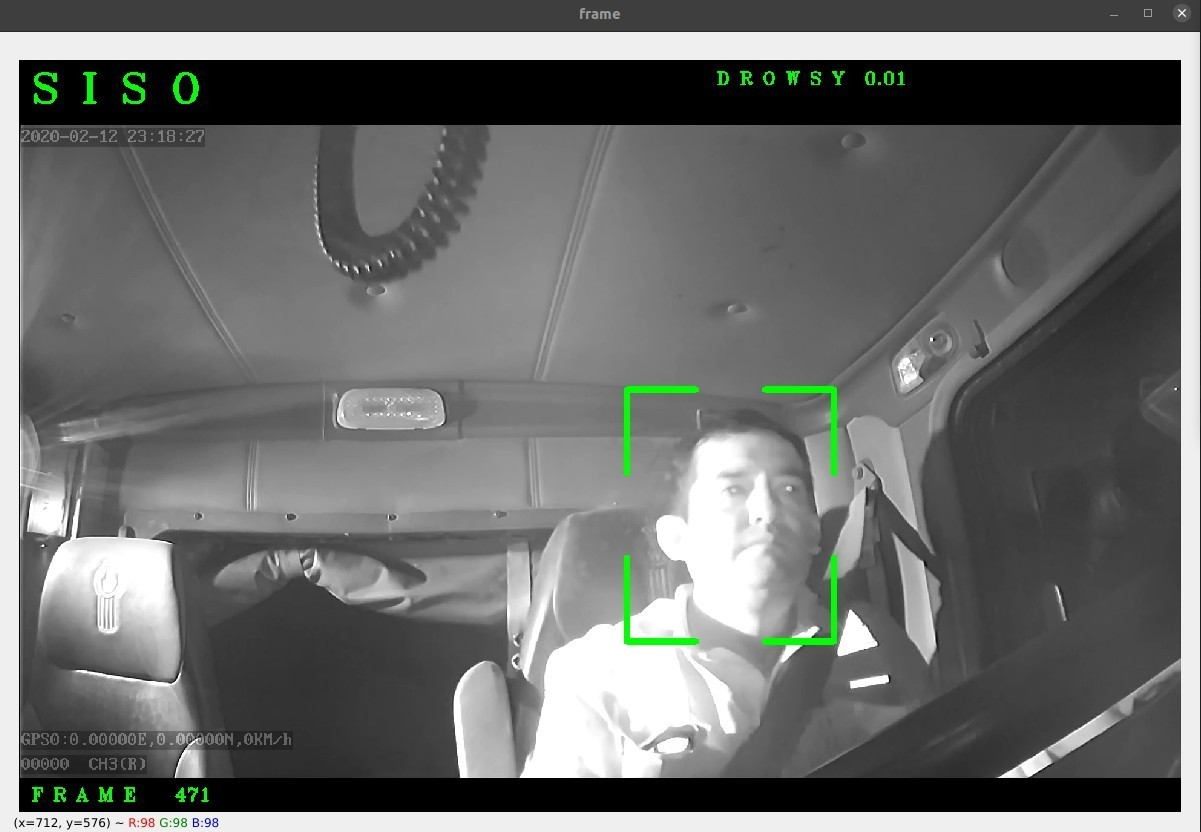
\includegraphics[width=0.5\textwidth,keepaspectratio]{img/sisi_vid1}\par 
			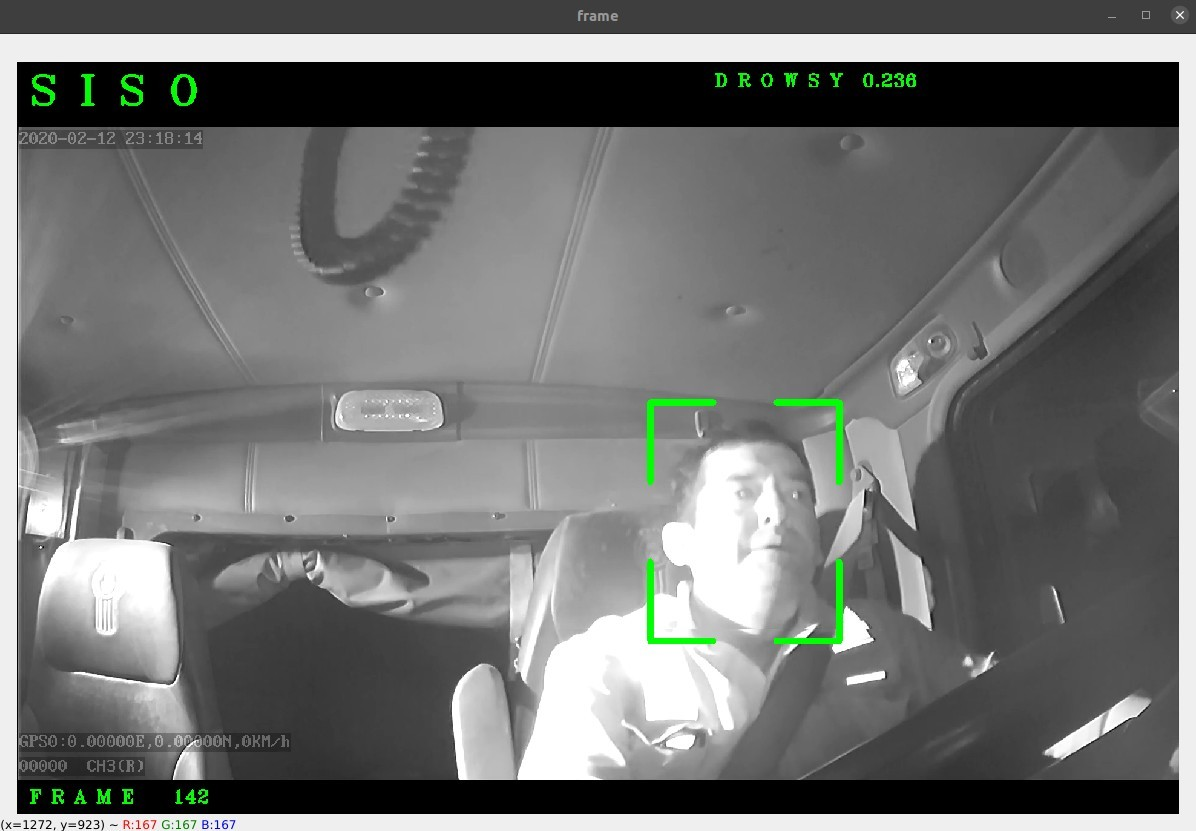
\includegraphics[width=0.5\textwidth,keepaspectratio]{img/sisi_vid2}\par 
			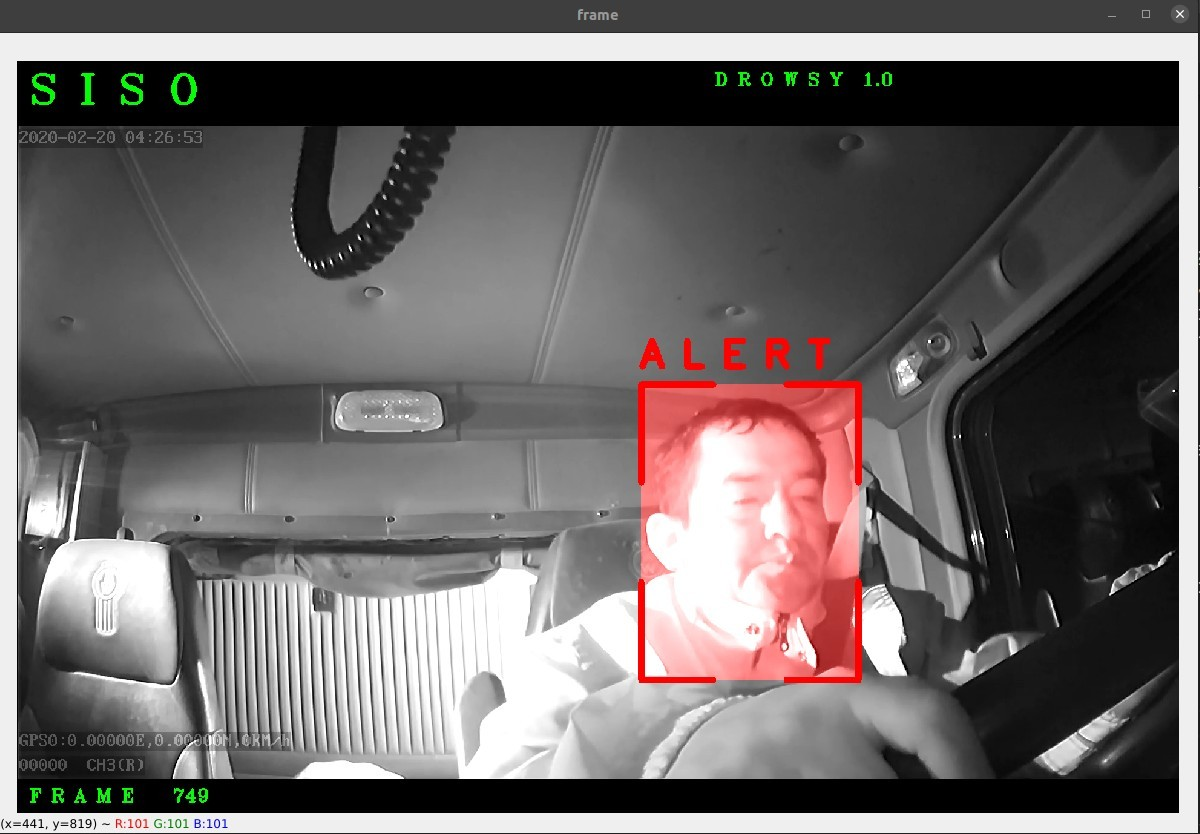
\includegraphics[width=0.5\textwidth,keepaspectratio]{img/sisi_vid7}\par 
			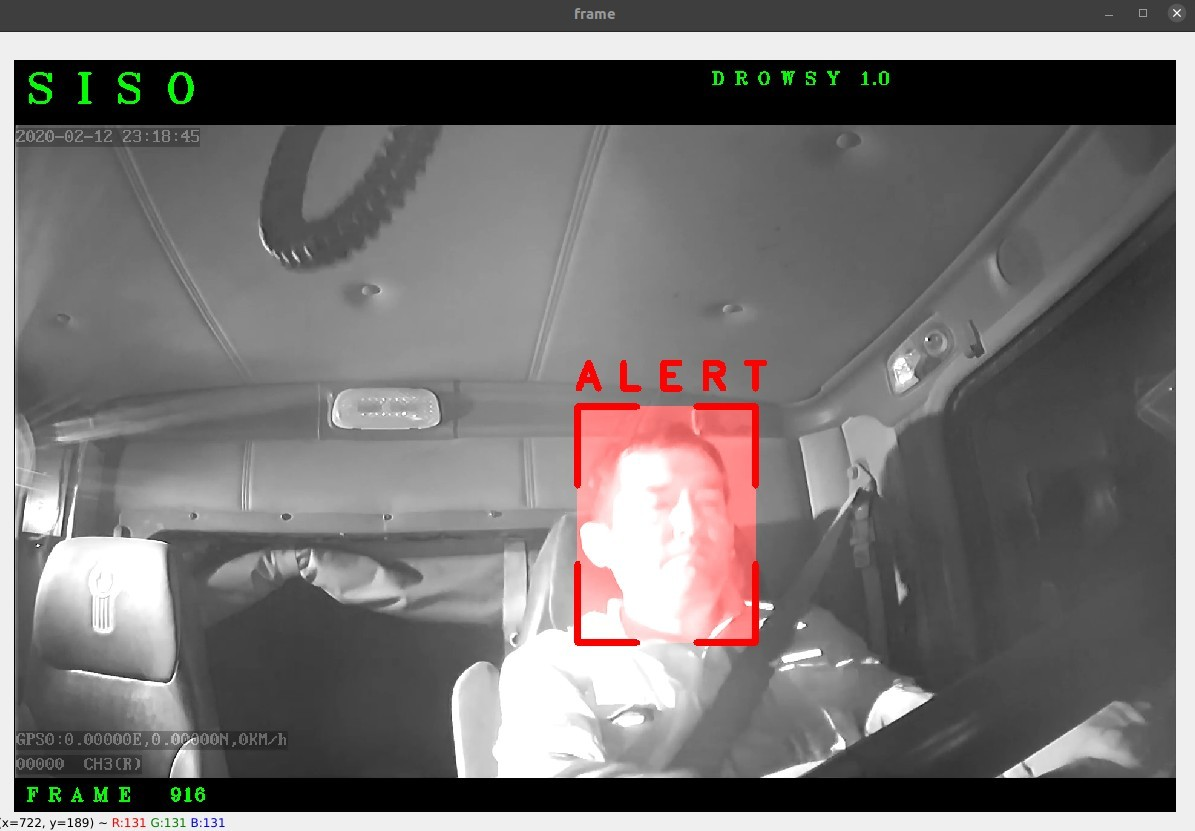
\includegraphics[width=0.5\textwidth,keepaspectratio]{img/sisi_vid8}\par 
		\end{multicols}
		\caption{SISO-VID en ejecución en la base de datos creada para el proyecto.}
		\label{img:siso_siso}
\end{figure}


	\begin{figure}[H]
		\centering
		\begin{multicols}{2}
			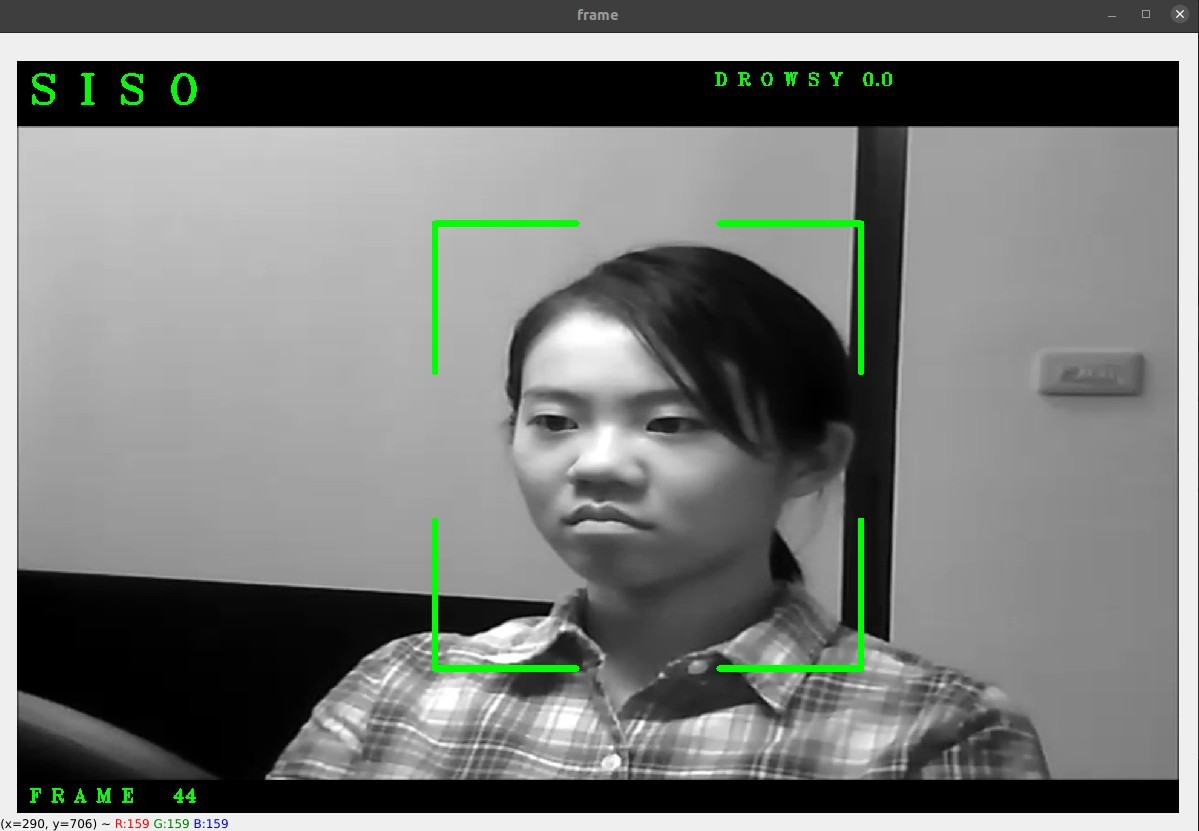
\includegraphics[width=0.5\textwidth,keepaspectratio]{img/sisi_vid9}\par 
			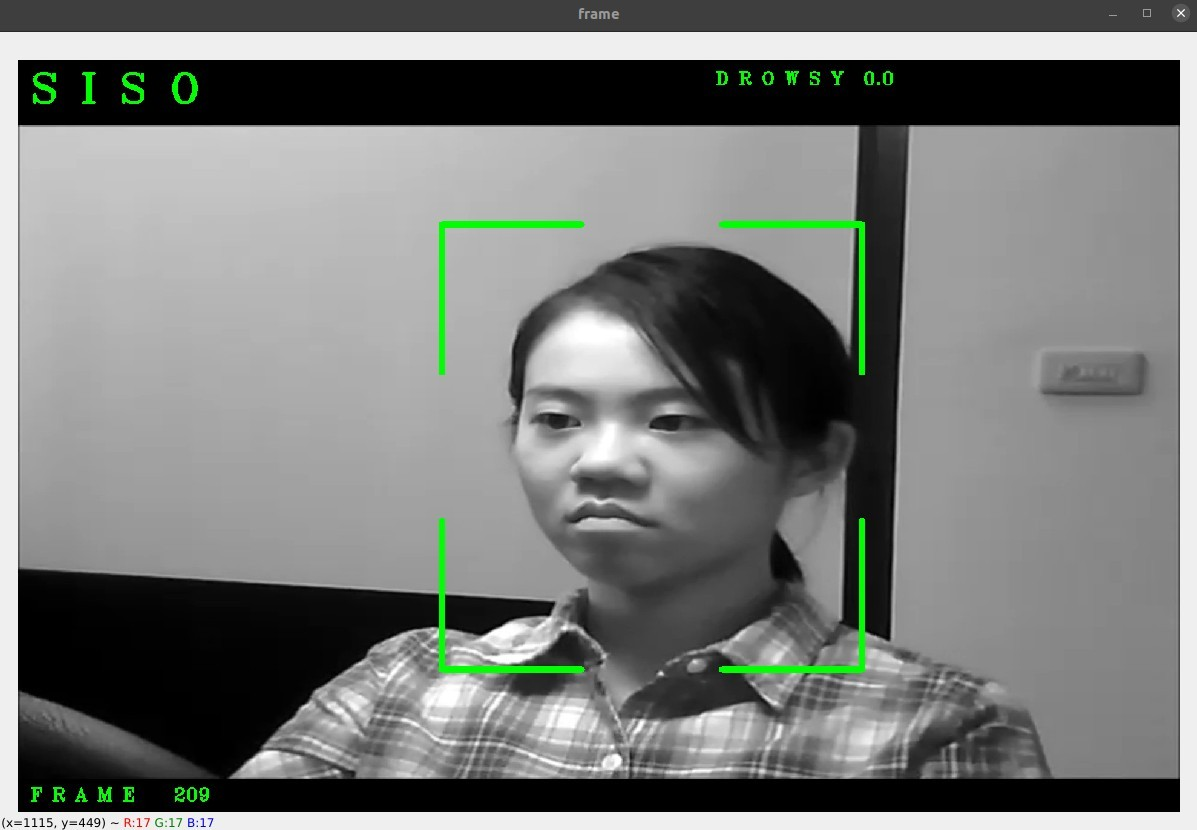
\includegraphics[width=0.5\textwidth,keepaspectratio]{img/sisi_vid10}\par 
			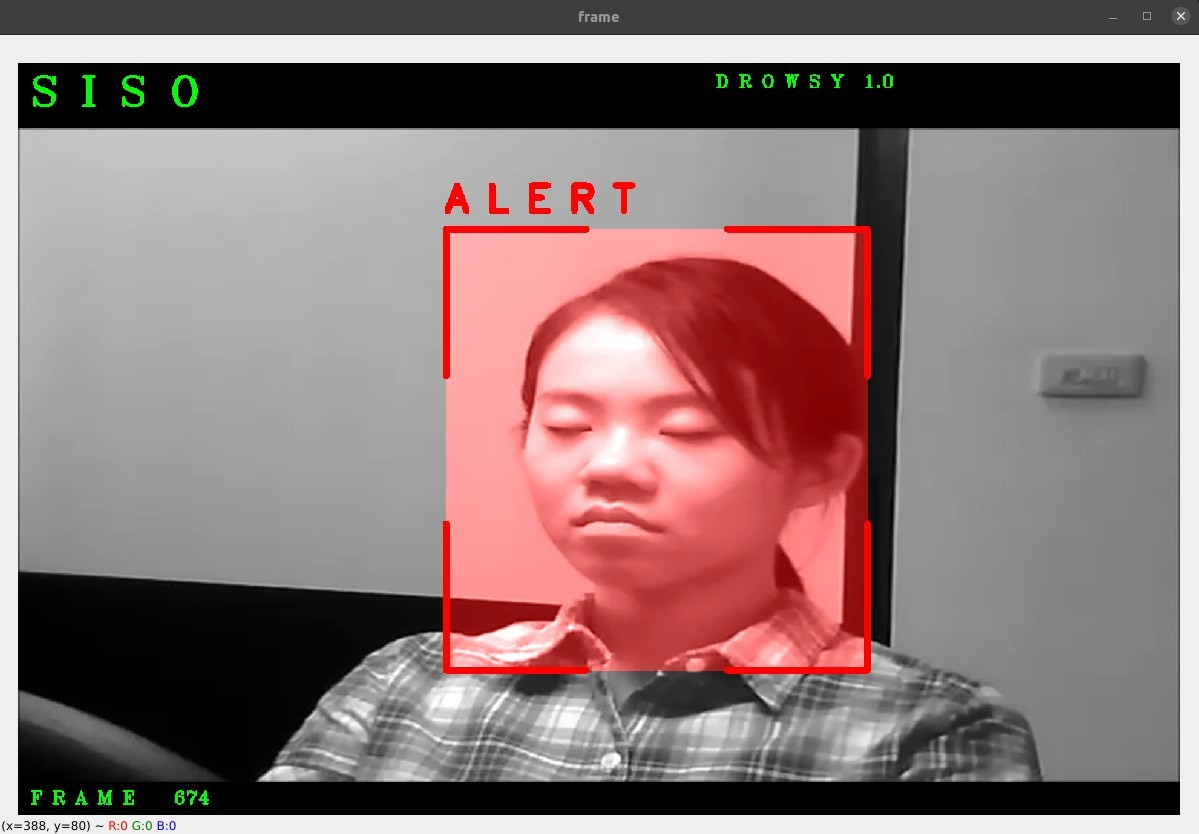
\includegraphics[width=0.5\textwidth,keepaspectratio]{img/sisi_vid11}\par 
			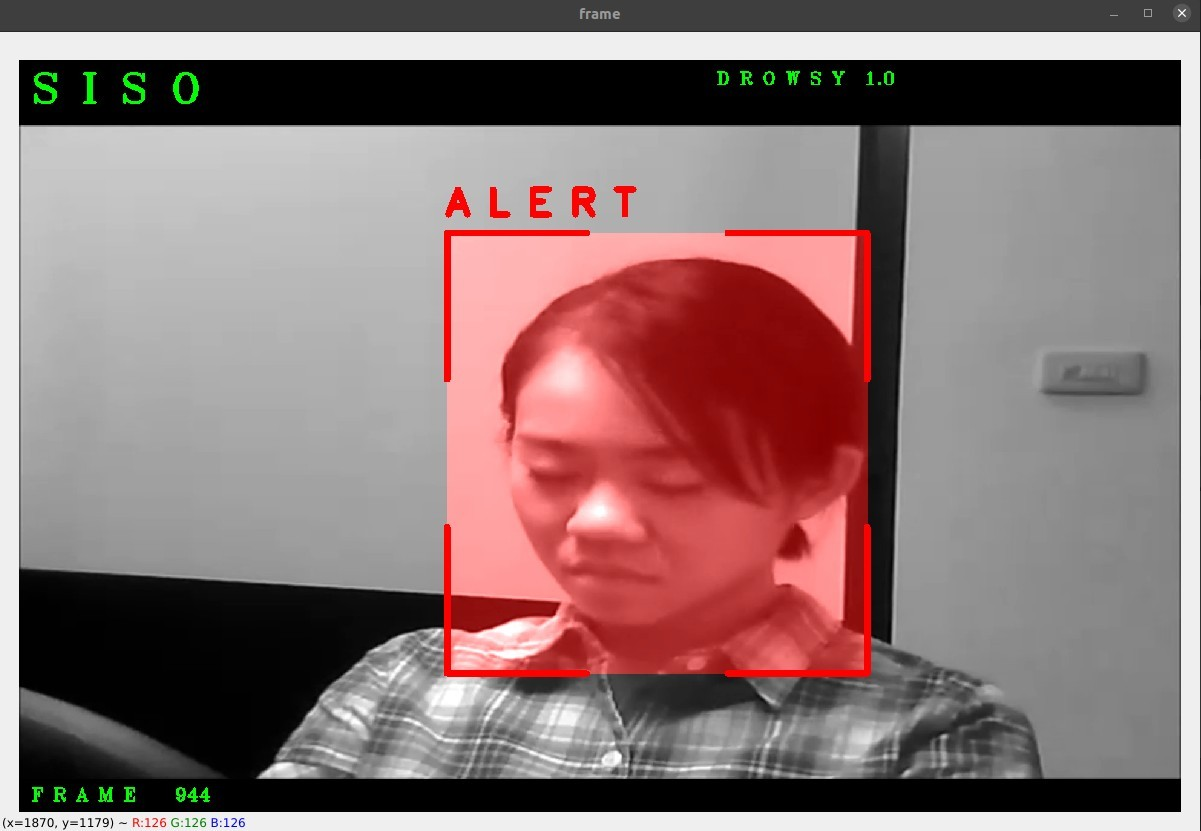
\includegraphics[width=0.5\textwidth,keepaspectratio]{img/sisi_vid12}\par 
		\end{multicols}
		\caption{SISO-VID en ejecución en la base de datos NTHU.}
		\label{img:siso_nthu}
	\end{figure}
	
	
	\section{Conclusiones}
	En este informe se a detallado las pruebas realizadas para la detección de somnolencia a partir de la imagen del rostro del conductor. Las pruebas consistieron en evaluar el desempeño de tres redes neuronales: VGG-16, ResNet e Inception-v3. Se evaluo el desempeño de cada red en tres bases de datos: NTHU, SISO-IMG y SISO-NTHU.\\
	
	En todas las bases de datos, la red neuronal Inception-v3 obtuvo el mejor desempeño, con un acierto de 87\% en la base de datos SISO-NTHU, 88\% en la base de datos NTHU y 96\% en la base de datos SISO-IMG. Esto demostro, que es factible detectar somnolencia utilizando aprendizaje profundo, incluso en entornos reales (SISO-IMG).\\


	%\clearpage
	
	\begin{table}[H]
	\begin{center}
			
	%\caption{Artículos de detección de somnolencia con procesamiento de video.}
	%\label{tab:comportameinto}
	\setlength{\tabcolsep}{0.5em} % for the horizontal padding
	{\renewcommand{\arraystretch}{1.4}% for the vertical padding
		
	\begin{tabular}{|p{1.6cm}|p{3cm}|p{3.5cm}|x{3.5cm}|p{2cm}|}
		\hline
		& \textbf{Nombre}    & \textbf{Cargo}         & \textbf{Firma} & \textbf{Fecha} \\ \hline
		\multirow{3}{1.6cm}{Elaborado por:} & Jason Paul Cahuana Nina        & Equipo técnico - Tesista La Salle    &  \raisebox{-.7\height}{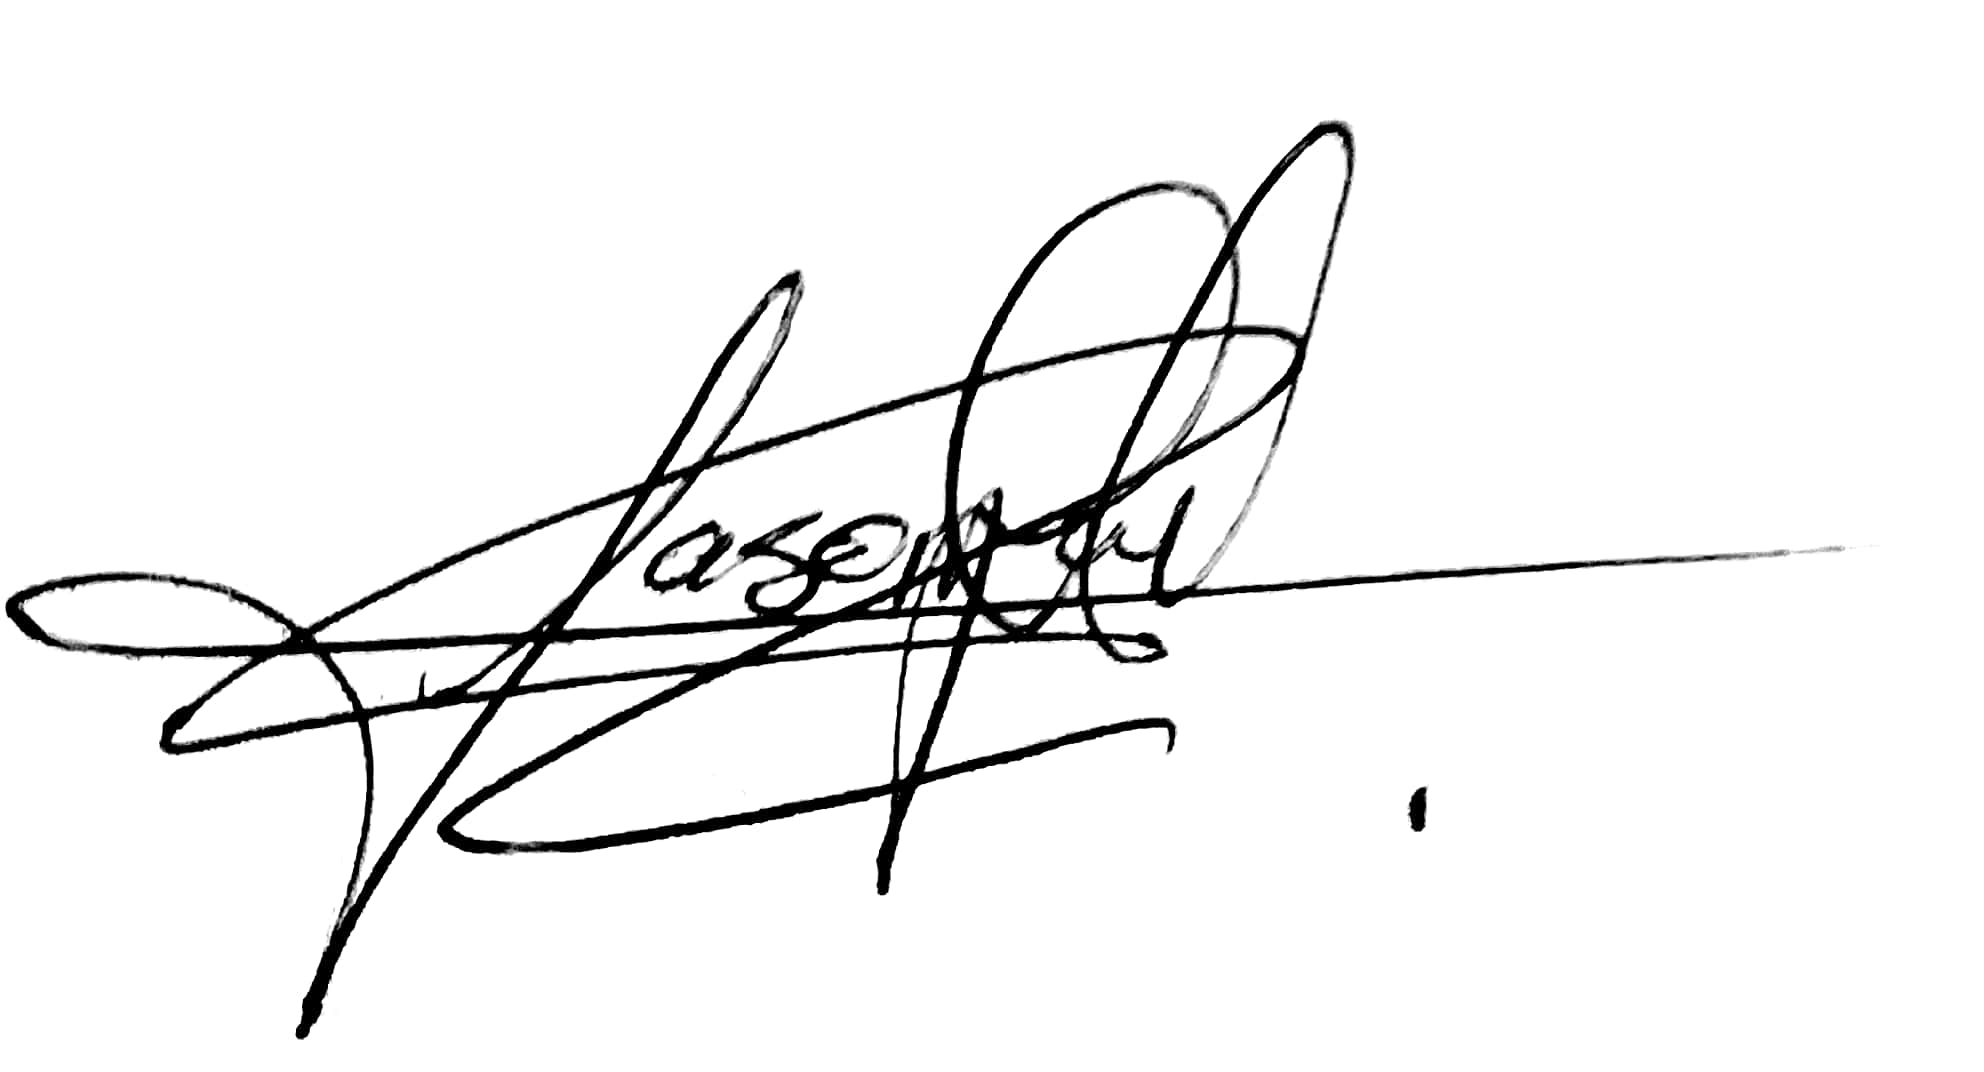
\includegraphics[width=2cm]{img/paul_firma.jpeg}}   &  12/03/2021     \\ \cline{2-5}		
		& Karla Mariel Fernández Fabián  & Investigador y desarrollador - Área de innovación y desarrollo tecnológico &  \raisebox{-.7\height}{
\includegraphics[width=2cm]{img/firma_KMFF}}     &   12/03/2021    \\ \hline
		
		& Vicente Enrique Machaca Arceda & Investigador y desarrollador - Área de innovación y desarrollo tecnológico &  \raisebox{-.7\height}{
\includegraphics[width=2cm]{img/firma_vicente}}     &   12/03/2021    \\ \hline
		
		\multirow{2}{1.6cm}{Revisado por:}  & Medardo Delgado Paredes        & Investigador La Salle  &  
			\raisebox{-.5\height}{
\includegraphics[width=2.5cm]{img/firma_yayo}}    &   12/03/2021    \\ \cline{2-5}	
		& Antonio Simon Bolivar Paredes  & Coordinador administrativo del proyecto    &     &  12/03/2021   \\ \hline
		Aprobado por:   & Elvis Diego Supo Colquehuanca  & Coorinador general del proyecto   &     &   12/03/2021   \\ \hline
	\end{tabular}

	}
	\end{center}
	\end{table}
	
	
	
	\clearpage
	\bibliographystyle{apalike}
	%\bibliographystyle{IEEEtranN}
	\bibliography{bibliography}
	
	
	\vspace*{\fill}
	
	

	
\end{document}
